\documentclass[14pt]{extarticle}
\usepackage[english,ukrainian]{babel}
\usepackage[utf8]{inputenc}
\usepackage[T1]{fontenc}

\usepackage{amsmath,amssymb}
\usepackage{parskip}
\usepackage{graphicx}
\usepackage{xcolor}
\usepackage{tcolorbox}
\tcbuselibrary{skins}
\usepackage[framemethod=tikz]{mdframed}
\usepackage{chngcntr}
\usepackage{enumitem}
\usepackage{hyperref}
\usepackage{float}
\usepackage{subfig}
\usepackage{esint}
\usepackage[top=2.5cm, left=3cm, right=3cm, bottom=4.0cm]{geometry}
\usepackage[table]{xcolor}
\usepackage{algorithm}
\usepackage{algpseudocode}
\usepackage{listings}

\title{Домашня робота з курсу ``Теоретична механіка''}
\author{Студента 3 курсу групи МП-31 Захарова Дмитра}
\date{\today}

\begin{document}

\maketitle

\section*{Завдання 12.28}

\textbf{Умова.} Нитка, прикріплена одним кінцем до тіла $A$ вагою $P$ (рис. \ref{fig:1}), яке рухається з тертям по горизонтальній площині, перекинута через нерухомий блок $C$, огинає рухомий блок $B$ вагою $Q$ і радіуса $r$ і закріплена другим кінцем $O$. Визначити швидкість $v$ тіла $A$ як функцію переміщення $s$ центра блока $B$, якщо момент інерції останнього відносно центра мас дорівнює $I$, коефіцієнт тертя тіла $A$ об площину дорівнює $\mu$.

\begin{figure}[H]
    \centering
    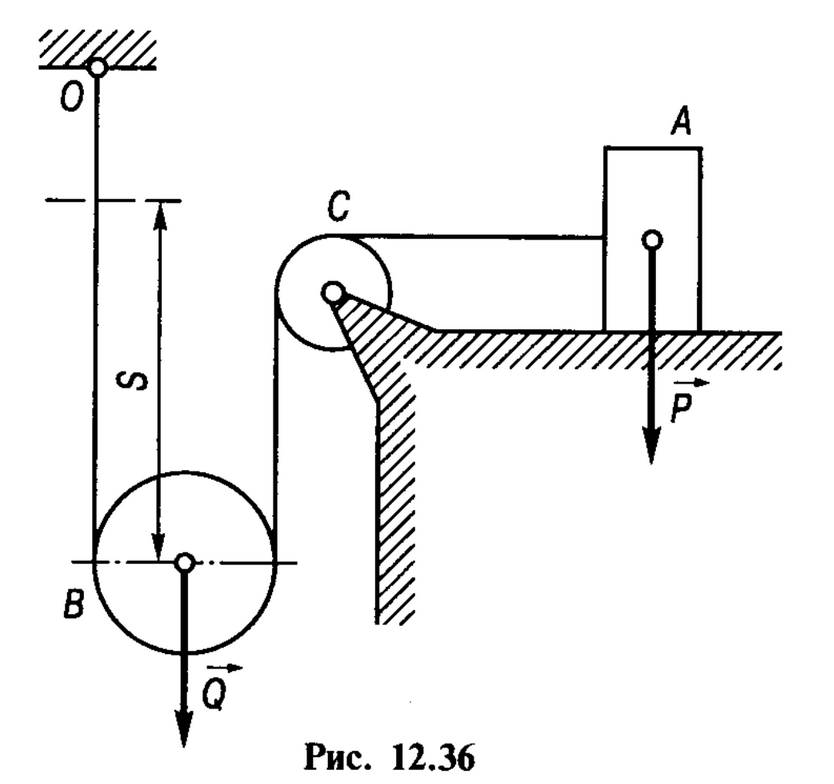
\includegraphics[width=0.4\textwidth]{images/hw_11/12-28.png}
    \caption{Умова до завдання 12.28}
    \label{fig:1}
\end{figure}

\textbf{Розв'язок.} Нехай блок змістився на $s$. Це означає, що груз змістився на $2s$, тобто робота сили тертя дорівнює $A_f=2\mu Ps$. Окрім цього, потенціальна енергія рухомого блоку змінилася на $\Delta W_p = Qs$.

Оскільки блок проходить вдвічі меньшу відстань, ніж груз, то лінійна швидкість блоку $\frac{v}{2}$. Це означає, що його кутова швидкість $\omega=\frac{v}{2r}$, а тому кінетична енергія обертання $\frac{I\omega^2}{2} = \frac{Iv^2}{8r^2}$. Отже, повна кінетична енергія системи:
\[
W_k = \frac{Q}{g} \cdot \frac{v^2}{8} + \frac{Iv^2}{8r^2} + \frac{P}{g} \cdot \frac{v^2}{2} = \left(\frac{Q+4P}{g} + \frac{I}{r^2}\right)\frac{v^2}{8}
\]
Вона перейшла у зміну потенціальної мінус сили тертя, тобто:
\[
\left(\frac{Q+4P}{g} + \frac{I}{r^2}\right)\frac{v^2}{8} = Qs - 2\mu P s
\]
Таким чином:
\[
v^2 = \frac{8s(Q-2\mu P)}{\frac{Q+4P}{g}+\frac{I}{r^2}} = \frac{8gsr^2(Q-2\mu P)}{(Q+4P)r^2 + Ig}
\]
Остаточно:
\[
\boxed{v = 2r\sqrt{\frac{2gs(Q-2\mu P)}{(Q+4P)r^2+Ig}}}
\]

\pagebreak
\section*{Завдання 12.32}

\textbf{Умова.} Колесо $1$ масою $M$ може котитися без ковзання у вертикальній площині всередині нерухомої шестерні $2$; воно приводиться в рух кривошипом $AB$ завздовжки $L$ і масою $m$. У початковий момент кут $\alpha$ між кривошипом і вертикальною віссю складав $\pi/3$. Кривошип відпустили без початкової швидкості. Визначити його кутову швидкість у момент проходження положення рівноваги. Тертям знехтувати.

\begin{figure}[H]
    \centering
    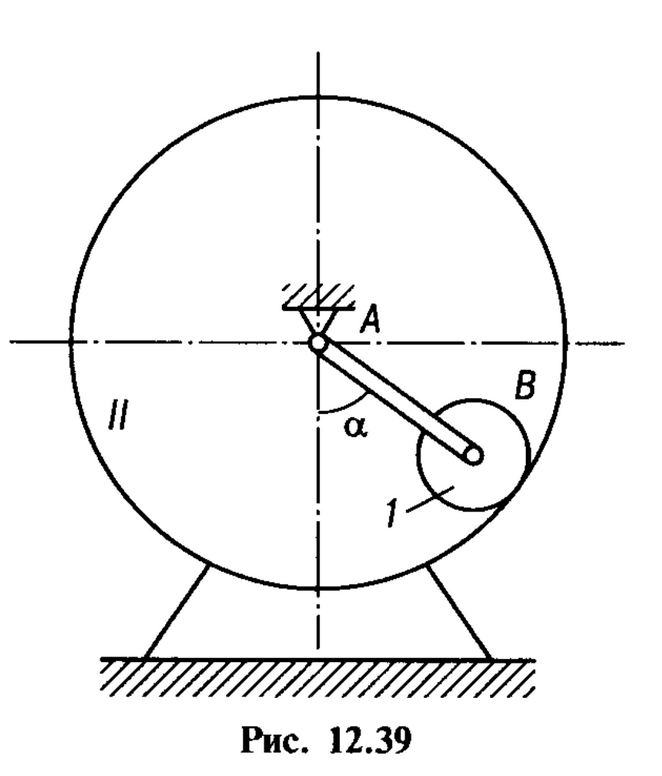
\includegraphics[width=0.5\textwidth]{images/hw_11/12-32.png}
    \caption{Умова до завдання 12.32}
    \label{fig:2}
\end{figure}

\textbf{Розв'язок.} Візьмемо точку $A$ за нульовий рівень. Тоді початкова енергія системи дорівнює потенціальній енергії і дорівнює:
\[
W_p = -\frac{mgL}{2}\cos\alpha - MgL \cos\alpha = -gL\cos\alpha\left(\frac{m}{2}+M\right)
\]
У момент проходження нижньої точки потенціальна енергія стає:
\[
W_p' = -gL\left(\frac{m}{2} + M\right)
\]
Таким чином, зміна потенціальної енергії:
\[
\Delta W_p = W_p' - W_p = -gL\left(\frac{m}{2}+M\right)(1-\cos\alpha) = -(m+2M)gL \sin^2 \frac{\alpha}{2}
\]
Ця потенціальна енергія пішла на зміну кінетичної. Спочатку її не було. В кінці ж швидкість набуває і стрижень, і кривошип. Момент інерції стрижня відносно $A$ дорівнює $\frac{1}{3}mL^2$, а у колеса, якщо вважати, що його радіус $R$, $I_{B} = MR^2$. В такому разі кінетична енергія стрижня $\frac{I_{AB}\omega^2}{2} = \frac{m\omega^2L^2}{6}$. 

Розбираємось з колесом. Лінійна швидкість колеса дорівнює $\omega L$, тому кутова швидкість самого колеса $\omega L = \Omega R$, отже $\Omega = \frac{L}{R}\cdot \omega$. Кінетична енергія в такому разі $\frac{M\omega^2L^2}{2}+\frac{I_B\Omega^2}{2} = \frac{M\omega^2L^2}{2}+\frac{MR^2L^2\omega^2}{2R^2}=M\omega^2L^2$ -- як бачимо, від радіуса колеса нічого не залежить. Отже, загальна кінетична енергія:
\[
W_k = \frac{m\omega^2 L^2}{6} + M\omega^2 L^2 = \left(\frac{m}{6} + M\right)\omega^2L^2
\]
Прирівнюємо вираз від'ємної зміни потенціальної енергії до прибутку кінетичної:
\[
\left(\frac{m}{6}+M\right)\omega^2 L^2 = (m+2M)gL \sin^2 \frac{\alpha}{2}
\]
Звідси остаточно:
\[
\boxed{\omega^2 = \frac{m+2M}{m+6M} \cdot \frac{6g\sin^2\frac{\alpha}{2}}{L}}
\]

\textit{Замітка.} Якщо вважати колесо суцільним, то його момент інерції $\frac{1}{2}MR^2$ і в такому разі загальна кінетична енергія колеса $\frac{3}{2}M\omega^2 L^2$. Це приводить до відповіді
\[
\omega^2 = \frac{m+2M}{m+9M} \cdot \frac{6g\sin^2\frac{\alpha}{2}}{L}
\]

\end{document}

